\documentclass[twoside]{book}

% Packages required by doxygen
\usepackage{calc}
\usepackage{doxygen}
\usepackage{graphicx}
\usepackage[utf8]{inputenc}
\usepackage{makeidx}
\usepackage{multicol}
\usepackage{multirow}
\usepackage{textcomp}
\usepackage[table]{xcolor}

% Font selection
\usepackage[T1]{fontenc}
\usepackage{mathptmx}
\usepackage[scaled=.90]{helvet}
\usepackage{courier}
\usepackage{amssymb}
\usepackage{sectsty}
\renewcommand{\familydefault}{\sfdefault}
\allsectionsfont{%
  \fontseries{bc}\selectfont%
  \color{darkgray}%
}
\renewcommand{\DoxyLabelFont}{%
  \fontseries{bc}\selectfont%
  \color{darkgray}%
}

% Page & text layout
\usepackage{geometry}
\geometry{%
  a4paper,%
  top=2.5cm,%
  bottom=2.5cm,%
  left=2.5cm,%
  right=2.5cm%
}
\tolerance=750
\hfuzz=15pt
\hbadness=750
\setlength{\emergencystretch}{15pt}
\setlength{\parindent}{0cm}
\setlength{\parskip}{0.2cm}
\makeatletter
\renewcommand{\paragraph}{%
  \@startsection{paragraph}{4}{0ex}{-1.0ex}{1.0ex}{%
    \normalfont\normalsize\bfseries\SS@parafont%
  }%
}
\renewcommand{\subparagraph}{%
  \@startsection{subparagraph}{5}{0ex}{-1.0ex}{1.0ex}{%
    \normalfont\normalsize\bfseries\SS@subparafont%
  }%
}
\makeatother

% Headers & footers
\usepackage{fancyhdr}
\pagestyle{fancyplain}
\fancyhead[LE]{\fancyplain{}{\bfseries\thepage}}
\fancyhead[CE]{\fancyplain{}{}}
\fancyhead[RE]{\fancyplain{}{\bfseries\leftmark}}
\fancyhead[LO]{\fancyplain{}{\bfseries\rightmark}}
\fancyhead[CO]{\fancyplain{}{}}
\fancyhead[RO]{\fancyplain{}{\bfseries\thepage}}
\fancyfoot[LE]{\fancyplain{}{}}
\fancyfoot[CE]{\fancyplain{}{}}
\fancyfoot[RE]{\fancyplain{}{\bfseries\scriptsize Generated on Wed Apr 22 2015 13\-:03\-:35 for Beer\-Me by Doxygen }}
\fancyfoot[LO]{\fancyplain{}{\bfseries\scriptsize Generated on Wed Apr 22 2015 13\-:03\-:35 for Beer\-Me by Doxygen }}
\fancyfoot[CO]{\fancyplain{}{}}
\fancyfoot[RO]{\fancyplain{}{}}
\renewcommand{\footrulewidth}{0.4pt}
\renewcommand{\chaptermark}[1]{%
  \markboth{#1}{}%
}
\renewcommand{\sectionmark}[1]{%
  \markright{\thesection\ #1}%
}

% Indices & bibliography
\usepackage{natbib}
\usepackage[titles]{tocloft}
\setcounter{tocdepth}{3}
\setcounter{secnumdepth}{5}
\makeindex

% Hyperlinks (required, but should be loaded last)
\usepackage{ifpdf}
\ifpdf
  \usepackage[pdftex,pagebackref=true]{hyperref}
\else
  \usepackage[ps2pdf,pagebackref=true]{hyperref}
\fi
\hypersetup{%
  colorlinks=true,%
  linkcolor=blue,%
  citecolor=blue,%
  unicode%
}

% Custom commands
\newcommand{\clearemptydoublepage}{%
  \newpage{\pagestyle{empty}\cleardoublepage}%
}


%===== C O N T E N T S =====

\begin{document}

% Titlepage & ToC
\hypersetup{pageanchor=false}
\pagenumbering{roman}
\begin{titlepage}
\vspace*{7cm}
\begin{center}%
{\Large Beer\-Me }\\
\vspace*{1cm}
{\large Generated by Doxygen 1.8.6}\\
\vspace*{0.5cm}
{\small Wed Apr 22 2015 13:03:35}\\
\end{center}
\end{titlepage}
\clearemptydoublepage
\tableofcontents
\clearemptydoublepage
\pagenumbering{arabic}
\hypersetup{pageanchor=true}

%--- Begin generated contents ---
\chapter{Hierarchical Index}
\section{Class Hierarchy}
This inheritance list is sorted roughly, but not completely, alphabetically\-:\begin{DoxyCompactList}
\item Test\-Case\begin{DoxyCompactList}
\item \contentsline{section}{db\-Doxygen.\-Test\-\_\-\-S\-Q\-L\-\_\-\-D\-B}{\pageref{classdbDoxygen_1_1Test__SQL__DB}}{}
\end{DoxyCompactList}
\end{DoxyCompactList}

\chapter{Class Index}
\section{Class List}
Here are the classes, structs, unions and interfaces with brief descriptions\-:\begin{DoxyCompactList}
\item\contentsline{section}{\hyperlink{classdbDoxygen_1_1Test__SQL__DB}{db\-Doxygen.\-Test\-\_\-\-S\-Q\-L\-\_\-\-D\-B} \\*Test class for testing database }{\pageref{classdbDoxygen_1_1Test__SQL__DB}}{}
\end{DoxyCompactList}

\chapter{Class Documentation}
\hypertarget{classdbDoxygen_1_1Test__SQL__DB}{\section{db\-Doxygen.\-Test\-\_\-\-S\-Q\-L\-\_\-\-D\-B Class Reference}
\label{classdbDoxygen_1_1Test__SQL__DB}\index{db\-Doxygen.\-Test\-\_\-\-S\-Q\-L\-\_\-\-D\-B@{db\-Doxygen.\-Test\-\_\-\-S\-Q\-L\-\_\-\-D\-B}}
}


Test class for testing database.  


Inheritance diagram for db\-Doxygen.\-Test\-\_\-\-S\-Q\-L\-\_\-\-D\-B\-:\begin{figure}[H]
\begin{center}
\leavevmode
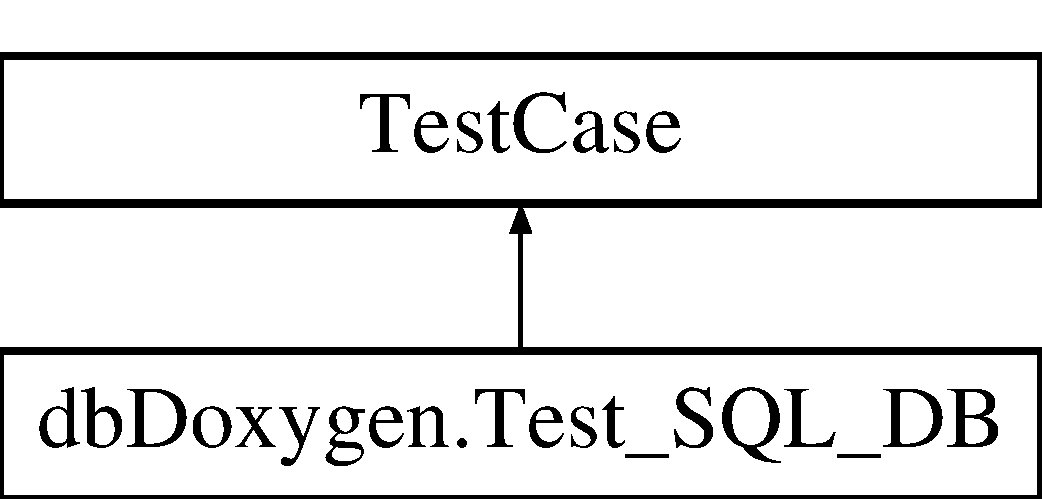
\includegraphics[height=2.000000cm]{classdbDoxygen_1_1Test__SQL__DB}
\end{center}
\end{figure}
\subsection*{Public Member Functions}
\begin{DoxyCompactItemize}
\item 
def \hyperlink{classdbDoxygen_1_1Test__SQL__DB_ae0d35ceea4631b889f44716107f4e52c}{Test\-Get\-Name\-Using\-Beer\-I\-D}
\begin{DoxyCompactList}\small\item\em Confirms that beer category I\-D's are linked to proper beer category names in Beer\-Cat table. \end{DoxyCompactList}\item 
def \hyperlink{classdbDoxygen_1_1Test__SQL__DB_a9f25d58b2c8ab5d6c6536a5dc7214a01}{Test\-Get\-Color\-Using\-Color\-I\-D}
\begin{DoxyCompactList}\small\item\em A method. \end{DoxyCompactList}\item 
def \hyperlink{classdbDoxygen_1_1Test__SQL__DB_a727a9b3476f267325da6a3d3f7442dc8}{Test\-Get\-Food\-Using\-Food\-I\-D}
\begin{DoxyCompactList}\small\item\em A method. \end{DoxyCompactList}\item 
def \hyperlink{classdbDoxygen_1_1Test__SQL__DB_a12f7edd9bde8e132987f8a095a419e9a}{Test\-Get\-Beer\-Name\-Using\-Food\-Id}
\begin{DoxyCompactList}\small\item\em A method. \end{DoxyCompactList}\item 
\hypertarget{classdbDoxygen_1_1Test__SQL__DB_a0b50d1b2d1920798ec59b26a0c538a29}{def \hyperlink{classdbDoxygen_1_1Test__SQL__DB_a0b50d1b2d1920798ec59b26a0c538a29}{Test\-Get\-Review\-Using\-Food\-Id\-And\-Beer}}\label{classdbDoxygen_1_1Test__SQL__DB_a0b50d1b2d1920798ec59b26a0c538a29}

\begin{DoxyCompactList}\small\item\em Doc for method. \end{DoxyCompactList}\end{DoxyCompactItemize}


\subsection{Detailed Description}
Test class for testing database. 

This class tests that S\-E\-L\-E\-C\-T statements return desired results. \begin{DoxyAuthor}{Authors}
Jacob C. Levine, Spencer Wilson, Matt Geckle 
\end{DoxyAuthor}

\begin{DoxyParams}{Parameters}
{\em unittest.\-Test\-Case} & The Test Case pointer. \\
\hline
\end{DoxyParams}


\subsection{Member Function Documentation}
\hypertarget{classdbDoxygen_1_1Test__SQL__DB_a12f7edd9bde8e132987f8a095a419e9a}{\index{db\-Doxygen\-::\-Test\-\_\-\-S\-Q\-L\-\_\-\-D\-B@{db\-Doxygen\-::\-Test\-\_\-\-S\-Q\-L\-\_\-\-D\-B}!Test\-Get\-Beer\-Name\-Using\-Food\-Id@{Test\-Get\-Beer\-Name\-Using\-Food\-Id}}
\index{Test\-Get\-Beer\-Name\-Using\-Food\-Id@{Test\-Get\-Beer\-Name\-Using\-Food\-Id}!dbDoxygen::Test_SQL_DB@{db\-Doxygen\-::\-Test\-\_\-\-S\-Q\-L\-\_\-\-D\-B}}
\subsubsection[{Test\-Get\-Beer\-Name\-Using\-Food\-Id}]{\setlength{\rightskip}{0pt plus 5cm}def db\-Doxygen.\-Test\-\_\-\-S\-Q\-L\-\_\-\-D\-B.\-Test\-Get\-Beer\-Name\-Using\-Food\-Id (
\begin{DoxyParamCaption}
\item[{}]{self}
\end{DoxyParamCaption}
)}}\label{classdbDoxygen_1_1Test__SQL__DB_a12f7edd9bde8e132987f8a095a419e9a}


A method. 


\begin{DoxyParams}{Parameters}
{\em self} & The object pointer. \\
\hline
\end{DoxyParams}
\hypertarget{classdbDoxygen_1_1Test__SQL__DB_a9f25d58b2c8ab5d6c6536a5dc7214a01}{\index{db\-Doxygen\-::\-Test\-\_\-\-S\-Q\-L\-\_\-\-D\-B@{db\-Doxygen\-::\-Test\-\_\-\-S\-Q\-L\-\_\-\-D\-B}!Test\-Get\-Color\-Using\-Color\-I\-D@{Test\-Get\-Color\-Using\-Color\-I\-D}}
\index{Test\-Get\-Color\-Using\-Color\-I\-D@{Test\-Get\-Color\-Using\-Color\-I\-D}!dbDoxygen::Test_SQL_DB@{db\-Doxygen\-::\-Test\-\_\-\-S\-Q\-L\-\_\-\-D\-B}}
\subsubsection[{Test\-Get\-Color\-Using\-Color\-I\-D}]{\setlength{\rightskip}{0pt plus 5cm}def db\-Doxygen.\-Test\-\_\-\-S\-Q\-L\-\_\-\-D\-B.\-Test\-Get\-Color\-Using\-Color\-I\-D (
\begin{DoxyParamCaption}
\item[{}]{self}
\end{DoxyParamCaption}
)}}\label{classdbDoxygen_1_1Test__SQL__DB_a9f25d58b2c8ab5d6c6536a5dc7214a01}


A method. 


\begin{DoxyParams}{Parameters}
{\em self} & The object pointer. \\
\hline
\end{DoxyParams}
\hypertarget{classdbDoxygen_1_1Test__SQL__DB_a727a9b3476f267325da6a3d3f7442dc8}{\index{db\-Doxygen\-::\-Test\-\_\-\-S\-Q\-L\-\_\-\-D\-B@{db\-Doxygen\-::\-Test\-\_\-\-S\-Q\-L\-\_\-\-D\-B}!Test\-Get\-Food\-Using\-Food\-I\-D@{Test\-Get\-Food\-Using\-Food\-I\-D}}
\index{Test\-Get\-Food\-Using\-Food\-I\-D@{Test\-Get\-Food\-Using\-Food\-I\-D}!dbDoxygen::Test_SQL_DB@{db\-Doxygen\-::\-Test\-\_\-\-S\-Q\-L\-\_\-\-D\-B}}
\subsubsection[{Test\-Get\-Food\-Using\-Food\-I\-D}]{\setlength{\rightskip}{0pt plus 5cm}def db\-Doxygen.\-Test\-\_\-\-S\-Q\-L\-\_\-\-D\-B.\-Test\-Get\-Food\-Using\-Food\-I\-D (
\begin{DoxyParamCaption}
\item[{}]{self}
\end{DoxyParamCaption}
)}}\label{classdbDoxygen_1_1Test__SQL__DB_a727a9b3476f267325da6a3d3f7442dc8}


A method. 


\begin{DoxyParams}{Parameters}
{\em self} & The object pointer. \\
\hline
\end{DoxyParams}
\hypertarget{classdbDoxygen_1_1Test__SQL__DB_ae0d35ceea4631b889f44716107f4e52c}{\index{db\-Doxygen\-::\-Test\-\_\-\-S\-Q\-L\-\_\-\-D\-B@{db\-Doxygen\-::\-Test\-\_\-\-S\-Q\-L\-\_\-\-D\-B}!Test\-Get\-Name\-Using\-Beer\-I\-D@{Test\-Get\-Name\-Using\-Beer\-I\-D}}
\index{Test\-Get\-Name\-Using\-Beer\-I\-D@{Test\-Get\-Name\-Using\-Beer\-I\-D}!dbDoxygen::Test_SQL_DB@{db\-Doxygen\-::\-Test\-\_\-\-S\-Q\-L\-\_\-\-D\-B}}
\subsubsection[{Test\-Get\-Name\-Using\-Beer\-I\-D}]{\setlength{\rightskip}{0pt plus 5cm}def db\-Doxygen.\-Test\-\_\-\-S\-Q\-L\-\_\-\-D\-B.\-Test\-Get\-Name\-Using\-Beer\-I\-D (
\begin{DoxyParamCaption}
\item[{}]{self}
\end{DoxyParamCaption}
)}}\label{classdbDoxygen_1_1Test__SQL__DB_ae0d35ceea4631b889f44716107f4e52c}


Confirms that beer category I\-D's are linked to proper beer category names in Beer\-Cat table. 

Test format\-: S\-E\-L\-E\-C\-T Name F\-R\-O\-M Beer\-Cat Where Beer\-Cat.\-Id=$<$\-I\-Dnumber$>$ 
\begin{DoxyParams}{Parameters}
{\em self} & The object pointer \\
\hline
\end{DoxyParams}


The documentation for this class was generated from the following file\-:\begin{DoxyCompactItemize}
\item 
db\-Doxygen.\-py\end{DoxyCompactItemize}

%--- End generated contents ---

% Index
\newpage
\phantomsection
\addcontentsline{toc}{chapter}{Index}
\printindex

\end{document}
